

\pdfoutput=1

\documentclass[envcountsame]{llncs}

\usepackage[utf8]{inputenc}

\usepackage[protrusion=true,expansion=true]{microtype}


\usepackage[style=numeric,
%  backref=true,
 isbn=false,
 maxnames=3,
 maxbibnames=99 ,                
 uniquename=init ,
]{biblatex}
\bibliography{literature.bib}

\usepackage{mdframed}
\usepackage{ownstylesansthm}

\usepackage{comment}
\excludecomment{Long}\includecomment{Short}
% \includecomment{Long}\excludecomment{Short}

\pagestyle{plain}

\begin{document}

\title{Terminal semantics for codata types\\in intensional Martin-L\"of type theory}

\author{Benedikt Ahrens and R\'egis Spadotti}

\institute{
Institut de Recherche en Informatique de Toulouse\\
Universit\'e Paul Sabatier, 
Toulouse}

\newcommand{\fat}[1]{\textbf{#1}}





\maketitle

% \tableofcontents

\begin{abstract}


 In this work, we study the notions of \emph{relative comonad} and \emph{comodule over a relative comonad}.
 We use these notions to give categorical semantics for the coinductive type families of streams and
 of infinite triangular matrices and their respective cosubstitution operations in intensional Martin-L\"of type theory.
 Our results are mechanized in the proof assistant \coq.
   
  
  \end{abstract}




\section{Introduction}
 
 In this work, we study the notions of \emph{relative comonad} and \emph{comodule over a relative comonad}.
 We then use these notions to characterize several coinductive data types and their respective cosubstitution operations 
 in intensional Martin-L\"of type theory via a universal property.
 
 In the following, we explain some of the vocabulary occurring in these first sentences.
 
\begin{Long}
 \subsection{About inductive types}
\end{Long}
\begin{Short}
 \paragraph*{About inductive types}
\end{Short}


 In a set-theoretic setting, inductive sets are characterized as initial algebras for 
 some endofunctor on the category of sets. For instance, the set of natural numbers constitutes the carrier of the 
 initial algebra of the functor $X \mapsto  \{ * \} \amalg X = 1 + X$.
 
 In a type-theoretic setting as given by Martin-L\"of type theory \parencite{martin_lof}, 
 two approaches to the semantics of inductive types have been studied: 
 one approach consists in showing that inductive types exist in a \emph{model} of the type theory,
 as is done, e.g., by \textcite{DBLP:journals/apal/MoerdijkP00}.
 Another approach is to prove that adding certain type-theoretic rules to the type theory---rules which postulate the existence
 of inductive types in the type theory---implies (or is equivalent to) the existence of a universal object \emph{within} type theory
 (see, e.g., \parencite{DBLP:conf/lics/AwodeyGS12, DBLP:journals/tcs/Dybjer97}).
 This latter approach is the one we adopt in the present work: we add axioms to intensional Martin-Löf type theory 
 which postulate the existence of \emph{co}inductive types, see below.
 
 Some attention has to be given to 
 the precise formulation of the type theory in question, in particular, to the nature of \emph{equality} in the type theory.
 There are two notions of equality in Martin-Löf type theory, an external (judgmental) one, and an internal (propositional) one.
 The latter is internalized by the \emph{identity type}, a type family that associates to any two 
 inhabitants $a,b : A$ of a type $A$ the type of (propositional) \enquote{identities} between them.
 Judgmentally equal terms are always propositionally equal, but the converse is not always true.
 One distinguishes two variants of type theory: in \emph{extensional} type theory, propositional equalities (i.e.\ terms of identity type)
 are reflected, via a \emph{reflection rule}, into the judgmental equality of the type theory.  
 Here, judgmental and propositional equality thus coincide.
 In \emph{intensional} type theory, there is no such reflection rule.
 
%  When specifying a universal property within type theory, one needs a suitable notion of \emph{uniqueness} (of certain maps or morphisms).
%  The property of uniqueness (or more generally, equality) of morphisms may now be expressed in terms of either judgmental or propositional equality.
%   While in extensional type theory the two equalities coincide, in intensional type theory they do not, making this choice a crucial one.
%  
 
 The reflection rule equips \emph{extensional} type theory with extensional features similar to those of set theory.
 As a consequence, the characterization given by \textcite{DBLP:journals/tcs/Dybjer97} of an inductive type in extensional MLTT as initial algebra for some endofunctor on the category of types  works as in the category of sets.
 
 
  

 Intensional Martin-L\"of type theory \parencite{martin_lof} lacks the reflection principle for the sake of decidability of type checking. 
 It forms the base of two computer proof assistants, \coq and \agda.
  The characterization of inductive types as initial algebras of some endofunctor in intensional Martin-Löf type theory fails \parencite{DBLP:journals/tcs/Dybjer97}, 
  but it can be recovered \parencite{DBLP:conf/lics/AwodeyGS12} in an \emph{extension} of intensional MLTT called
  \emph{Homotopy Type Theory} \parencite{hottbook}.
  In this extension, function extensionality is provable from the \emph{Univalence Axiom}. 
 For a suitable definition of \emph{uniqueness}---\emph{contractibility} in HoTT jargon---one can prove uniqueness of the
 algebra morphisms out of the one whose carrier is given by the inductive type under consideration.
 The mentioned work \parencite{DBLP:conf/lics/AwodeyGS12} thus shows that the characterization of inductive types as initial algebras carries over 
 from extensional to intensional type theory if one adds an extensionality principle for functions and adapts the notion of uniqueness.
 
 
 The characterization of inductive sets/types as initial objects in some category
 has been extended to some \emph{heterogeneous}---also called \emph{nested}---inductive data types, e.g., the type of $\lambda$-terms,
 in different formulations \parencite{fpt, DBLP:journals/iandc/HirschowitzM10}.
 The main goal of these works is not just to characterize a data type via a universal property, but rather a data type
 \emph{equipped with a canonical, well-behaved substitution operation}.
 
\begin{Long}
 \subsection{Coinductive types: simply dualizing?}
\end{Long}
\begin{Short}
 \paragraph*{Coinductive types: simply dualizing?}
\end{Short}

 
 In a traditional set-theoretic setting, the theory of coinductive sets is completely dual to that of inductive sets:
 dually to inductive sets, \emph{co}inductive sets such as streams are characterized as terminal coalgebras of 
 suitable endofunctors \parencite{jacobs1997tutorial}.
 
 In type theory, this duality between inductive and coinductive objects breaks. This is rooted in the 
 unsuitability of the Martin-Löf identity type to express sameness for inhabitants of coinductive types:
 while identity terms are inductively generated and hence necessarily finite, 
 a proof of sameness between coinductive terms---which represent infinite objects---constitutes a potentially infinite object itself.
 The type of such proofs hence cannot be exhaustively given by the (inductive) identity type.
 
 Instead of comparing two coinductive terms in Martin-Löf type theory up to identity, one defines a 
 binary coinductive relation called \emph{bisimilarity} on a given coinductive type, with respect to which one compares its inhabitants  \parencite{DBLP:conf/types/Coquand93}. 
 Categorically, this relation is given as the greatest---terminal---relation on the coinductive type that is compatible with the coalgebra structure.
 
 Consequently, we consider two maps into a coinductive type to be the same if they are \emph{pointwise bisimilar}---an analogue
 to the aforementioned principle of function extensionality available in Homotopy Type Theory. 
 With these conventions, we give, in the present work, a characterization of some coinductive data types as \emph{terminal} object in some category 
 defined in intensional Martin-L\"of type theory.
 More precisely, we consider an example of \emph{homogeneous} codata type, streams, and 
 an example of \emph{heterogeneous} codata type, triangular matrices.
 For each of these examples we prove, 
 from type-theoretic rules specifying the respective codata type added to the basic rules of Martin-L\"of type theory,
 the existence of a terminal object in some category \emph{within IMLTT}.
 The objects of the considered categories are not plain coalgebras for some endofunctor, but rather coalgebras with extra structure.
 This extra structure accounts for a \emph{cosubstitution} operation with which one can equip the considered codata types \emph{in a canonical way}.
 The cosubstitution operation is explained in the next section.
 
\begin{Long} 
 \subsection{Cosubstitution: a comonadic operation on parametrized codata}
\end{Long}
\begin{Short}
 \paragraph*{Cosubstitution: a comonadic operation on parametrized codata}
\end{Short}

 
 Many inductive types, in particular parametrized ones representing \emph{syntax} such as the lambda calculus, 
 are canonically equipped with a substitution operation. The categorical characterization of this substitution operation
 has been studied extensively; our list of pointers \parencite{alt_reus, fpt, Power:2007:ASS:1230146.1230276, Tanaka:2005:UCF:1088454.1088457,
 DBLP:journals/iandc/HirschowitzM10, DBLP:conf/fossacs/AltenkirchCU10, ahrens_relmonads} is necessarily incomplete.
 One such characterization is via \emph{monads}; substitution can be seen as part of a monadic structure on the functor 
 given by the parametrized data type \parencite{alt_reus, 
 DBLP:journals/iandc/HirschowitzM10, DBLP:conf/fossacs/AltenkirchCU10, ahrens_relmonads}.
 
 Dually, coinductive types can often be equipped with a \emph{cosubstitution} operation. 
 Is this cosubstitution operation part of a comonad structure?
 
 In a set-theoretic setting, the fact that cosubstitution for coinductive sets is comonadic is established by \textcite{DBLP:conf/sfp/UustaluV01}.
 
  
 In IMLTT however, 
 in order to characterize that cosubstitution operation on a given codata type, and its algebraic properties,
 we develop the notion of \emph{relative comonad} and \emph{comodule over a relative comonad}.
 The need to consider \emph{relative} comonads arises from the  need to check the algebraic properties of cosubstitution modulo \emph{bisimilarity} rather
 than modulo identity (in the sense of the Martin-Löf identity types).
 
 
 In order to integrate a notion of cosubstitution into the categorical semantics of the coinductive types under consideration,
 we do not consider a category of plain coalgebras for some endofunctor.
 Instead, we consider coalgebras with extra structure accounting for a comonadic operation, which for the terminal coalgebra
 is given by cosubstitution.
 Our terminal semantics characterizes not only the codata types themselves but also the bisimilarity relation 
 and---via the use of (relative) comonads---a canonical cosubstitution operation on them.
 
\begin{Long} 
 \subsection{Our proofs are correct}
\end{Long}
\begin{Short}
 \paragraph*{Our proofs are correct}
\end{Short}

 
 All our results have been implemented in the proof assistant \coq \parencite{coq84pl3}.
 The \coq source files and HTML documentation are available online \parencite{trimat_coq}.
 In this document, we hence omit the proofs and focus on definitions and statements of lemmas.
 
\begin{Short}
\paragraph*{A longer version} A longer version of this article is available on the arXiv \parencite{trimat_coq}.
 There, we give details we had to omit from this version for reasons of space: 
  we show how to get relative comonads from (traditional) comonads, 
           remark on relative comonads into cartesian closed categories,
           explain the relationship to coalgebra semantics, report on the formalization in \coq of our results and
           give proofs of the results in this work.
\end{Short}

 
 
 \subsubsection*{Disclaimer}The category-theoretic concepts studied in this work are agnostic to the foundational system being worked in.
 While we present them in a type-theoretic style, the definitions and lemmas can trivially be transferred to a set-theoretic setting.
 Throughout this article, we use type-theoretic notation,  writing $t:T$ to indicate that $t$ is of type $T$. 
 For instance, we write $f : \C(A,B)$ to indicate that $f$ is a morphism from object $A$ to object $B$ in category $\C$.
 Whenever an operation takes several arguments, we write some of them as indices; these indices might be omitted when 
 they can be deduced from the type of the later arguments.
 We assume basic knowledge of category theory; any instances used are defined in the following.
  
%  \subsubsection*{More related work}
 
% %  The notion of \emph{module over a monad}, which we dualize and generalize in this work, is used by \textcite{DBLP:journals/iandc/HirschowitzM10}
% %  to give an initial semantics result for languages with variable binding. 
%  Their work is based on work of \textcite{alt_reus},
%  who show that the lambda calculus equipped with a simultaneous substitution constitutes a monad.
%  We make use of the notion of \emph{relative comonad}, the dual to relative monads as introduced by \textcite{DBLP:conf/fossacs/AltenkirchCU10}.
%  One of our main examples, the codata type of infinite triangular matrices, is studied by \textcite{DBLP:conf/types/MatthesP11}.
%  Redecoration for both finite and infinite triangular matrices is used by \textcite{DBLP:journals/tcs/AbelMU05} to exemplify 
%  the expressivity of the studied recursion schemes.
 
\begin{Long}
 
 \subsubsection*{Organisation of the paper}
  In \Cref{sec:preliminaries} we introduce some concepts and notations used later on.
  In \Cref{sec:tri} we present the coinductive type families $\stream$ of streams and $\Tri$ of infinite triangular matrices and some operations on those codata types.
   Their specifying rules are given in \Cref{stream_rules} and \Cref{tri_rules}, respectively.
  In \Cref{sec:comonads} we present \emph{relative comonads} and define the category of comonads relative to a fixed functor.
    We give some examples of such structures, using the codata types presented in \Cref{sec:tri}.
  In \Cref{sec:comodules} we define comodules over relative comonads and give some constructions of comodules.
     Again, examples of such structures are taken from \Cref{sec:tri}.
  In \Cref{sec:coalgebras_for_tri} we define categories of models for the codata types presented in \Cref{sec:tri},
      based on the category-theoretic notions developed in the previous sections.
      We then prove that the codata types constitute the terminal model in the respective categories.
      Finally, we present an example of a map defined as a terminal map exploiting the universal property of streams.
  In \Cref{sec:formal} we explain some details of the formalization of this work in the proof assistant \coq.
  A table with the correspondence between formal and informal definitions is given in \Cref{sec:table_formal_informal}.

\end{Long}


\section{Preliminaries}\label{sec:preliminaries}

In this section we present some particular categories and functors used later on, and fix some notation.

\begin{definition}[Setoids in IMLTT]
  A \emph{setoid} in intensional Martin-Löf type theory is a pair $(A, \sim_A)$ of a type $A$ together with an equivalence 
  relation $\sim_A$ on $A$. Given a setoid $S = (A, \sim_A)$, we often abuse notation by writing $s:S$ instead of $s:A$ for
  a term $s$ of $A$.
  Given two setoids $(A,\sim_A)$ and $(B,\sim_B)$, the cartesian product $A\times B$ of their underlying types is equipped with
  an equivalence relation given component-wise, thus yielding a product on setoids.
\end{definition}



\begin{definition}[Category in IMLTT]\label{def:cat_imltt}
  A category $\C$ in intensional Martin-Löf type theory (see, e.g., \parencite{aczel_galois, concat}) is given by
  \begin{itemize}
   \item a type of objects, also denoted by $\C$;
   \item for any two objects $a,b:\C$, a \emph{setoid} $\C(a,b)$ of morphisms from $a$ to $b$;
   \item an identity morphism $\id_a : \C(a,a)$ for any $a:\C$;
   \item a dependent composition operation $(\comp{}{})_{a,b,c} : \C(b,c) \times \C(a,b) \to \C(a,c)$;
   \item a proof that composition is compatible with the equivalence relations of the setoids of morphisms;
   \item proofs of unitality and associativity of composition stated in terms of the equivalence relations on the morphisms.
  \end{itemize}
  We also write $f:a\to b$ for a morphism $f : \C(a,b)$, when the category $\C$ can be deduced from the context.
\end{definition}

Functors and natural transformations are defined in terms of the setoidal equivalence relations on morphisms.
We omit the definitions, which can be found in our \coq files.

\begin{definition}[Some categories]\label{def:set_setoid}
 We denote by $\Set$ the category (in IMLTT) of types (of a fixed universe) and total functions between them in Martin-L\"of type theory. 
 The setoidal equivalence relation on $\Set(A,B)$ is given by pointwise equality as given by the Martin-Löf identity type: 
   \[f \sim g \enspace =_{\text{def}} \enspace \forall x:A, fx = gx. \]
 
 We denote by $\Setoid$ the category an object of which is a setoid.
 A morphism between setoids is a type-theoretic function between the underlying types that is compatible in the obvious sense with the equivalence relations of the source and target setoids.
%  If $A$ is a setoid, we also use $A$ to refer to its underlying type, and thus write $a:A$ for an element $a$ of the type underlying the setoid $A$. 
%  We write $a\sim a'$ for related elements $a$ and $a'$ in $A$.
 The category $\Setoid$ is cartesian closed and hence a category in the sense of \Cref{def:cat_imltt}: 
 two parallel morphisms of setoids $f,g:A\to B$ are equivalent if for any $a:A$ we have $fa \sim_B ga$.
\end{definition}



\begin{definition}\label{def:eq}
 The functor $\eq : \Set\to\Setoid$ is defined as the left adjoint to the forgetful functor $U : \Setoid \to \Set$.
  Explicitly, the functor $\eq$ sends any type $X$ to the setoid $(X,=_X)$ given by the type $X$ itself, equipped
  with the propositional equality relation $=_X$ specified via Martin-L\"of's identity type on $X$.
\end{definition}


\begin{remark}[Notation for product]
  We denote the category-theoretic binary product of objects $A$ and $B$ of a category $\C$ by $A\times B$.
  We write $\pr_1(A,B) : \C(A\times B, A)$ and $\pr_2(A,B) :\C(A\times B, B)$ for the projections, occasionally omitting the 
  argument $(A,B)$.
  Given $f : \C(A, B)$ and $g : \C(A,C)$, we write $\langle f,g\rangle : \C(A,B\times C)$ for the induced map into the product such that
  $\comp{\langle f,g\rangle}{\pr_1} = f$ and $\comp{\langle f,g\rangle}{\pr_2} = g$.
\end{remark}

Both of the categories of \Cref{def:set_setoid} have finite products.

\begin{definition}\label{def:monoidal_functor}
 A functor $F:\C\to\D$ between categories with finite products \emph{preserves products} if, for any two objects $A$ and $B$ of $\C$,
  the morphism
 \[ \phi^F_{A,B} := \bigl\langle F(\pr_1), F(\pr_2) \bigr\rangle : \D\bigl(F(A\times B), FA\times FB\bigr)\enspace  \] 
 is an isomorphism.
\end{definition}

\begin{example}
  The functor $\eq: \Set \to \Setoid$ of \Cref{def:eq} preserves products.
\end{example}


\section{Codata types in intensional Martin-L\"of type theory}\label{sec:tri}

We consider two particular coinductive type families in Intensional Martin-L\"of type theory (IMLTT) \parencite{martin_lof}, 
a type-theoretic foundational system.
For $a,b : A$, we denote by $a = b$ the Martin-L\"of identity type between $a$ and $b$.

In this section, we present these types, and we also define \emph{bisimilarity} for each codata type.
Bisimilarity is a coinductively defined equivalence relation on types which is considered 
to be the appropriate notion of sameness on inhabitants of these types \parencite{DBLP:conf/types/Coquand93, DBLP:journals/corr/abs-cs-0603119}.
A coinductive type with bisimilarity hence forms a setoid as in \Cref{def:set_setoid}.
We thus denote bisimilar elements using an infix $\sim$, as in $t \sim t'$. 

% Maps into a coinductive data type are specified by the observations, i.e.\ the value of the destructors, on the output of those maps.  
% The precise rule for specifying maps into the considered coinductive type is given in \Cref{stream_rules}.




% In this text, we use a more convenient syntax, as illustrated in \Cref{eq:tail_sredec}.

The first example is the type of \emph{streams} of elements of a given base type $A$:
% In the presentation we use the notational convention of \Cref{def:set_setoid}, using the same name for a setoid and its underlying type.
\begin{example}\label{ex_stream}
  Let $A$ be a type. The type $\stream A$ of \emph{streams over $A$} is coinductively defined via the destructors 
  given in \Cref{stream_rules}.
  Intuitively, a map into streams is defined by specifying the observations---$\shead$ and $\stail$---on the output of that map: this intuition
  can be obtained by considering the combination of introduction and computation rules from \Cref{stream_rules}.
  We thus use a kind of \enquote{copattern matching} to define maps, as follows: 
  the clauses $\comp{f}{\shead} := h$ and $\comp{f}{\stail}:= t$ define $f := \corec(h,t)$.
  A more formal theory of copattern matching is developed by \textcite{DBLP:conf/popl/AbelPTS13}.
  We define a \emph{co}substition operation 
   \[\sredec_{A,B} : (\stream A \to B) \to \stream A\to\stream B\] 
   on streams via the following clauses:
% 
   \begin{align} \comp{\sredec~f}{\shead} := f \quad\text{ and } \quad
                  \comp{\sredec~f}{\stail} := \comp{\stail}{\sredec~f} \enspace . \label{eq:tail_sredec}
    \end{align}
  We call such an operation \enquote{cosubstitution} since its type is dual to, e.g., the simultaneous substitution operation 
  of the lambda calculus \parencite{alt_reus}.

\begin{figure}
 \begin{mdframed}
  
% \section{Rules for $\stream$ and bisimilarity}\label{stream_rules}

\paragraph*{Rules for $\stream$}



\begin{description}

 \item[Formation]\hfill \\
\mbox{\hfill} 
 \begin{center}
 \def\extraVskip{3pt}
     \def\proofSkipAmount{\vskip.8ex plus.8ex minus.4ex}

         
   \AxiomC{$A : \Set$}
    \UnaryInfC{$\stream A : \Set$}
     \DisplayProof
 \end{center} 
\mbox{\hfill}
\mbox{\hfill}
 \item[Elimination]\hfill \\
\mbox{\hfill}
\begin{center}
    \AxiomC{$t : \stream A$} %\doubleLine
     \UnaryInfC{$\shead_A~t : A$}
      \DisplayProof
                        \hspace{3ex}
                                       \AxiomC{$t : \stream A$}%\doubleLine
                                       \UnaryInfC{$\stail_A~t : \stream A$}
                                       \DisplayProof%
\end{center}
\mbox{\hfill}
\mbox{\hfill}
  \item[Introduction]\hfill \\                                     
\mbox{\hfill}
  \begin{center}
               \AxiomC{$T : \Set$} \AxiomC{$hd : T \to A$} \AxiomC{$tl : T \to T$} %\doubleLine
               \TrinaryInfC{$\corec_A~hd~tl : T \to \stream A$}
               \DisplayProof%
\end{center}
\mbox{\hfill}
\mbox{\hfill}         
  \item[Computation]\hfill \\
\mbox{\hfill}
\begin{center}          
               \AxiomC{$hd : T \to A$} \AxiomC{$tl : T \to T$} \AxiomC{$t:T$}%\doubleLine
               \TrinaryInfC{$\shead_A(\corec_A~hd~tl~t) = hd(t)$}
               \DisplayProof
               
               \vspace{1em}
               
               \AxiomC{$hd : T \to A$} \AxiomC{$tl : T \to T$} \AxiomC{$t:T$}%\doubleLine
               \TrinaryInfC{$\stail_A(\corec_A~hd~tl~t) = \corec_A~hd~tl~(tl~t)$}
               \DisplayProof
\end{center}

 \end{description}              
               
\paragraph*{Bisimilarity on $\stream$} %\label{stream_bisim}          
 

 
\begin{description}

 \item[Formation]\hfill \\
\mbox{\hfill} 
 \begin{center}
 \def\extraVskip{3pt}
     \def\proofSkipAmount{\vskip.8ex plus.8ex minus.4ex}

         
   \AxiomC{$A : \Set$} \AxiomC{$s, t : \stream A$}
    \BinaryInfC{$\bisim_A~s~t : \Set$}
     \DisplayProof
 \end{center} 
\mbox{\hfill}
\mbox{\hfill}
 \item[Elimination]\hfill \\
 \mbox{\hfill}
\begin{center}
    \AxiomC{$s, t : \stream A$} \AxiomC{$p: \bisim_A~s~t$} %\doubleLine
     \BinaryInfC{$\shead_A~s = \shead_A~t$}
      \DisplayProof
                        \hspace{3ex}
                                       \AxiomC{$s,t : \stream A$} \AxiomC{$p: \bisim_A~s~t$}%\doubleLine
                                       \BinaryInfC{$\bisim_A (\stail_A~s) (\stail_A~t)$}
                                       \DisplayProof%
\end{center}
\mbox{\hfill}
\mbox{\hfill}
  \item[Introduction]\hfill \\                                     
\mbox{\hfill}                        
\begin{center}

\def\fCenter{~\mbox{$\entails$}}
\def\ScoreOverhang{30pt}

               \Axiom$\fCenter\ R : \stream A \to \stream A \to \Set$ \noLine\UnaryInf$x,y : \stream A \fCenter\ R~x~y \to \shead~x = \shead~y$ \noLine
                \UnaryInf$x,y : \stream A \fCenter\ R~x~y \to R~(\stail~x) (\stail~y)$  %\doubleLine
               \UnaryInf$x,y : \stream A \fCenter\ R~x~y \to \bisim~x~y$
               \DisplayProof%
\end{center}
                      
%           \vspace{1em}


 \end{description}              
               
               
               
 \end{mdframed}
 \caption{Rules for streams and bisimilarity on them} \label{stream_rules}
\end{figure}

% 

\begin{comment}
  \begin{figure}[bt]
  \centering

     \def\extraVskip{3pt}
     \def\proofSkipAmount{\vskip.8ex plus.8ex minus.4ex}
    \AxiomC{$t : \stream A$} %\doubleLine
     \UnaryInfC{$\shead_A~t : A$}
      \DisplayProof
                        \hspace{3ex}
                                       \AxiomC{$t : \stream A$}%\doubleLine
                                       \UnaryInfC{$\stail_A~t : \stream A$}
                                       \DisplayProof%
% 
% 
% \vspace{2ex}
% 
\hspace{3ex}
 \centering
                                            \def\extraVskip{3pt}
     \def\proofSkipAmount{\vskip.8ex plus.8ex minus.4ex}
    \AxiomC{$t \sim t'$} %\doubleLine
     \UnaryInfC{$\shead~t = \shead~t'$}
      \DisplayProof
                        \hspace{3ex}
                                       \AxiomC{$t \sim t'$} %\doubleLine
                                       \UnaryInfC{$ \stail~t \sim \stail~t'$}
                                       \DisplayProof   
%   \end{center}
  \caption{Destructors and bisimilarity for the coinductive family $\stream$} \label{fig:stream_destructors}
\end{figure}
\end{comment}
   

\end{example}


\begin{Long}

Streams are node-labeled trees where every node has exactly one subtree.
We also consider a type of trees where every node has an arbitrary, but fixed, number of subtrees, 
parametrized by a type $B$.



\begin{example}[Node-labeled trees]\label{ex_trees}
 We denote by $\Tree_B(A)$ the codata type given by one destructor $\shead$ and a family of 
 destructors $(\stail_b)_{b:B}$ with types analogous to those defining $\stream$ of \Cref{ex_stream}.
 We thus obtain $\stream$ by considering, for $B$, the singleton type.
\end{example}

\end{Long}

Another codata type we consider models
\emph{infinite triangular matrices}. It is more sophisticated than the type of streams as one of its destructors is \emph{heterogeneous}:

\begin{example}\label{ex_tri}
The codata type of infinite triangular matrices is studied in detail by
 \textcite{DBLP:conf/types/MatthesP11}, and also by \textcite{DBLP:journals/tcs/AbelMU05}.
 We give a brief summary, but urge the reader to consult the given reference 
 for an in-depth explanation. 
 The codata type family $\Tri$ of infinite triangular matrices 
 is parametrized by a fixed type $E$ for entries not on the diagonal, 
 and indexed by another, \emph{variable}, type $A$ for entries on 
 the diagonal. 
\begin{Long}
 Schematically, such a matrix looks like in \Cref{fig_tri}.
 \begin{figure}[bt]
 \centering
 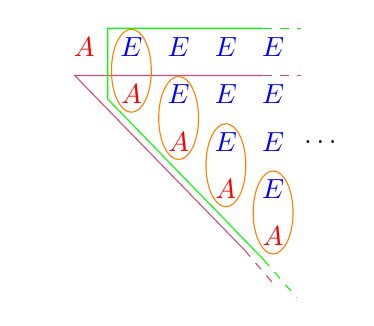
\begin{tikzpicture}[scale = 0.6]
    \foreach \y in {0,...,2}
    {\foreach \x in {\y,...,2}
      \draw (\x+1, -\y) node[color=blue]{$E$} ;
    }
    \foreach \x in {-1,...,3} \draw (\x, -\x-1) node[color=red]{$A$} ;
    \foreach \x in {0,...,3} \draw (\x, -\x)
    node[color=blue]{\textbf{$E$}} ;
    \draw(4,-2) node{$\ldots$};
    
    
      \draw[color=purple!70]  (2.4, -4.3) --node[auto, swap, left]{$\cut$}
     (-1.2,-0.6) -- (2.8,-0.6);
    \draw[color=purple!70, dashed]  (2.8,-0.6) -- (3.6,-0.6);
    \draw[color=purple!70, dashed]  (2.4,-4.3) -- (3.0,-5);

    \draw (-2,0) node{$\head$} ;
    

    \draw[color=green] (2.8,0.4) -- (-0.5,0.4) -- (-0.5, -1.1) --node[auto, swap, left]{$\tail$}
    (2.8,-4.5)  ; 
    \draw[color=green, dashed] (2.8,0.4) -- (3.6,0.4) ; 
    \draw[color=green, dashed] (2.8,-4.5) -- (3.5,-5.3) ; 


    \draw[color=orange](0, -0.5) ellipse (12pt and 25pt) ;  
    \draw[color=orange](1, -1.5) ellipse (12pt and 25pt) ;  
    \draw[color=orange](2, -2.5) ellipse (12pt and 25pt) ;  
    \draw[color=orange](3, -3.5) ellipse (12pt and 25pt) ;  
  \end{tikzpicture}\\[-2ex]
  \caption{An infinite triangular matrix over type $A$ and various operations}\label{fig_tri}
 \end{figure}
\end{Long}
% 
 It is specified via two destructors $\head$ and $\tail$, whose types are given in \Cref{tri_rules}.
\begin{Long}
 Given a matrix over type $A$, its $\tail$---obtained by removing the first element on the diagonal, i.e.\ the $\head$ element---can 
 be considered as a trapezium as indicated by the green line in \Cref{fig_tri}, or alternatively, as
 a triangular matrix over type $E\times A$, by bundling the entries of the diagonal with those above as indicated by the orange frames in \Cref{fig_tri}.
 The latter representation is reflected in the type of the destructor $\tail$.
\end{Long}
\begin{Short}
 Given a matrix over type $A$, its $\tail$---obtained by removing the first element on the diagonal, i.e.\ the $\head$ element---can 
 be considered as a trapezium or, alternatively, as a triangular matrix over type $E\times A$, 
 by bundling the entries of the diagonal with those directly above the diagonal.
\end{Short}

 Bisimilarity on the inhabitants of that type is defined via the destructors of \Cref{tri_rules}.    
 As with streams, we denote by $\Tri A$ not only the resulting \emph{setoid} of triangular matrices over $A$, but also its
 underlying \emph{type}. 
 
 \begin{figure}
 \begin{mdframed}
  
% \section{Rules for $\Tri$ and bisimilarity}\label{tri_rules}

\paragraph*{Rules for $\Tri$}

\begin{description}

 \item[Formation]\hfill \\
 
 \begin{center}
 \def\extraVskip{3pt}
     \def\proofSkipAmount{\vskip.8ex plus.8ex minus.4ex}

         
   \AxiomC{$A : \Set$}
    \UnaryInfC{$\Tri A : \Set$}
     \DisplayProof
 \end{center} 
 
 \item[Elimination]\hfill \\
 

%   \hspace{3ex}

\begin{center}
    \AxiomC{$t : \Tri A$} %\doubleLine
     \UnaryInfC{$\head_A~t : A$}
      \DisplayProof
                        \hspace{3ex}
                                       \AxiomC{$t : \Tri A$}%\doubleLine
                                       \UnaryInfC{$\tail_A~t : \Tri(E\times A)$}
                                       \DisplayProof%
\end{center}
  \item[Introduction]\hfill \\                                     
                       
%           \vspace{1em}             
            
\begin{center}
               \AxiomC{$T : \Set\to\Set$} 
               \AxiomC{$hd : \forall A,TA \to A$} \AxiomC{$tl : \forall A, T A \to T(E\times A)$} %\doubleLine
               \TrinaryInfC{$\corec_T~hd~tl :  \forall A, T A \to \Tri A$}
               \DisplayProof%
\end{center}
                      
%           \vspace{1em}
  \item[Computation]\hfill \\

\begin{center}          
               \AxiomC{$hd : \forall A,TA \to A$} \AxiomC{$tl : \forall A, T A \to T(E\times A)$} %\doubleLine
               \AxiomC{$t : TA$}
               \TrinaryInfC{$\head_T(\corec_A~hd~tl~t) = hd(t)$}
               \DisplayProof
               
               \vspace{1em}
               
               \AxiomC{$hd : \forall A,TA \to A$} \AxiomC{$tl : \forall A, T A \to T(E\times A)$} %\doubleLine
               \AxiomC{$t : TA$}
               \TrinaryInfC{$\tail_T(\corec_A~hd~tl~t) = \corec_A~hd~tl~(tl~t)$}
               \DisplayProof
\end{center}

 \end{description}              
               
\paragraph*{Bisimilarity for $\Tri$}              
 


               
 \begin{description}

 \item[Formation]\hfill \\
 
 \begin{center}
 \def\extraVskip{3pt}
     \def\proofSkipAmount{\vskip.8ex plus.8ex minus.4ex}

         
   \AxiomC{$A : \Set$} \AxiomC{$s, t : \Tri A$}
    \BinaryInfC{$\bisim_A~s~t : \Set$}
     \DisplayProof
 \end{center} 
 
 \item[Elimination]\hfill \\
 

%   \hspace{3ex}

\begin{center}
    \AxiomC{$s, t : \Tri A$} \AxiomC{$p: \bisim_A~s~t$} %\doubleLine
     \BinaryInfC{$\head_A~s = \head_A~t$}
      \DisplayProof
                        \hspace{3ex}
                                       \AxiomC{$s,t : \Tri A$} \AxiomC{$p: \bisim_A~s~t$}%\doubleLine
                                       \BinaryInfC{$\bisim_A (\tail_A~s) (\tail_A~t)$}
                                       \DisplayProof%
\end{center}
  \item[Introduction]\hfill \\                                     
                       
%           \vspace{1em}             
            
\begin{center}
               \AxiomC{$R : \forall A, \Tri A \to \Tri A \to \Set$} \noLine
               \UnaryInfC{$\forall A,\forall~s,t : \Tri A, R~s~t \to \head~s = \head~t$} \noLine
                \UnaryInfC{$\forall  A,\forall~s,t : \Tri A, R~s~t \to R~(\stail~s) (\stail~t)$}  %\doubleLine
               \UnaryInfC{$\forall A,\forall~s,t : \Tri A, R~s~t \to \bisim~s~t$}
               \DisplayProof%
\end{center}

\end{description}
               
 \end{mdframed}
 \caption{Rules for triangular matrices and bisimilarity on them} \label{tri_rules}
\end{figure}
 

\begin{comment}
\begin{figure}[bt]
  \centering

     \def\extraVskip{3pt}
     \def\proofSkipAmount{\vskip.8ex plus.8ex minus.4ex}
    \AxiomC{$t : \Tri~A$} %\doubleLine
     \UnaryInfC{$\head_A~t : A$}
      \DisplayProof
                        \hspace{3ex}
                                       \AxiomC{$t : \Tri~A$}%\doubleLine
                                       \UnaryInfC{$\tail_A~t : \Tri(E\times A)$}
                                       \DisplayProof%
% 
% 
% \vspace{2ex}
% 
 \hspace{3ex}
                                            \def\extraVskip{3pt}
     \def\proofSkipAmount{\vskip.8ex plus.8ex minus.4ex}
    \AxiomC{$t \sim t'$}%\doubleLine
     \UnaryInfC{$\head~t = \head~t'$}
      \DisplayProof
                        \hspace{3ex}
                                       \AxiomC{$t \sim t'$}%\doubleLine
                                       \UnaryInfC{$ \tail~t \sim \tail~t'$}
                                       \DisplayProof   

  \caption{Destructors and bisimilarity for the coinductive family $\Tri$} \label{fig:tri_destructors}
\end{figure}
\end{comment}
% 
% 
  A cosubstitution operation, \enquote{redecoration},
    $ \redec_{A,B} : (\Tri A \to B) \to \Tri A \to \Tri B$
  is defined  through the clauses
% 
  \begin{align} \comp{\redec~f}{\head} := f \quad\text{ and } \quad
                  \comp{\redec~f}{\tail} := \comp{\tail}{\redec~(\extend~f)} \enspace . \label{eq:rest_redec}
    \end{align}
Here, the family of functions 
     $\extend_{A,B} : (\Tri A \to B) \to \Tri (E \times A) \to E\times B $
  is suitably defined to account for the change of the type of the argument of $\redec$ when redecorating $\tail~t : \Tri(E\times A)$
  rather than $t : \Tri A$, namely
  \[ \extend(f) := \langle \comp{\head_{E\times A}}{\pr_1(E,A)} , \comp{\cut_A}{f} \rangle \enspace . \]
  The auxiliary function $\cut_A : \Tri(E\times A) \to \Tri A$ is defined corecursively via
% 
  \begin{align*} \comp{\cut}{\head} := \comp{\head}{\pr_2} \quad\text{ and } \quad
                     \comp{\cut}{\tail} := \comp{\tail}{\cut} \enspace . 
      \end{align*}
%       
All the operations are suitably compatible with the bisimilarity relations, so that they can be equipped with the types
  \begin{align*}
    \redec_{A,B} &: \Setoid(\Tri A,\eq B) \to \Setoid(\Tri A,\Tri B ) \\
    \extend_{A,B} &: \Setoid(\Tri A,\eq B) \to \Setoid\bigr(\Tri (E \times A),\eq(E\times B)\bigr) \\
    \cut_A &:  \Setoid(\Tri(E\times A) , \Tri A) \enspace .
  \end{align*}
\end{example}

\begin{Long}
Note how heterogeneity of the destructor $\tail$ makes the definition of $\redec$ considerably more complicated than that of
the analogous operation $\sredec$ on streams.
\end{Long}

  
\section{Relative comonads and their morphisms}\label{sec:comonads}

In this section we define the category of \emph{comonads relative to a fixed functor}, and present some examples 
of such comonads and their morphisms.

\emph{Relative monads} were defined by \textcite{DBLP:conf/fossacs/AltenkirchCU10} as a notion of monad-like structure
whose underlying functor is not necessarily an endofunctor.
The dual notion is that of a relative \emph{co}monad:

\begin{definition}%[Relative comonad]
 \label{def:rel_comonad}
  Let $F:\C\to\D$ be a functor. A \fat{relative comonad $T$ over $F$} is given by
  \begin{packitem}\setlength{\itemsep}{.7em}
   \item a map $T:\C_0 \to \D_0$ on the objects of the categories involved;
   \item an operation $\counit : \forall A : \C_0, \D(TA,FA)$;
   \item an operation $\cobind: \forall A,B:\C_0, \D(TA,FB) \to \D(TA,TB)$
%   \end{packitem}
   such that
%   \begin{packitem}
   \item $\forall A,B:\C_0, \forall f:\D(TA,FB), \comp{\cobind(f)}{\counit_B} = f$;
   \item $\forall A : \C_0, \cobind(\counit_A) = \id_{TA}$;
   \item $\forall A,B,C:\C_0, \forall f : \D(TA,FB),\forall g:\D(TB,FC), \\
        \comp{\cobind(f)}{\cobind(g)} = \cobind(\comp{\cobind(f)}{g})$.
  \end{packitem} 
\end{definition}

\begin{Short}
\begin{remark}\label{def:lift}
 \begin{itemize}
  \item Relative comonads over the identity functor are comonads.
  \item Just like relative monads, relative comonads are functorial.
  \item Under some conditions on the functor $F$, one can obtain comonads relative to $F$ from (absolute) comonads on the 
 source category $\C$.
  \item A \emph{weak constructive comonad} as defined by \textcite{DBLP:conf/types/MatthesP11}  is \emph{precisely}
  a comonad relative to the functor $\eq : \Set\to\Setoid$.
 \end{itemize}
\noindent
Details are given in the long version of this article \parencite{trimat_coq}.
\end{remark}
\end{Short}


\begin{Long}
Just like relative monads, relative comonads are functorial:
\begin{definition}%[Functoriality for relative comonads]
\label{def:lift}
 Let $T$ be a  comonad relative to $F:\C\to\D$.
 For $f : \C(A,B)$ we define
  $ \lift^T(f) := \cobind(\comp{\counit_A}{Ff}) : \D(TA,TB)$. 
 The functor properties are easily checked.
\end{definition}

\begin{remark}
 It follows from the comonadic axioms that
 counit and cobind are natural transformations with respect to the functoriality defined in \Cref{def:lift}:
 \begin{align*}
     \counit &: T \to F : \C\to \D \\
     \cobind &: \D(T\_, F\_) \to \D(T\_, T\_) : \C^{\text{op}} \times \C \to \Ens \enspace .
 \end{align*}

\end{remark}


\end{Long}

\begin{Long}
Relative comonads over the identity functor are exactly comonads.
\end{Long}



\begin{Long}

\begin{example}[Relative comonads from comonads]\label{ex_relcom_from_com}
  Let $F : \C \to \D$ be a fully faithful functor and $(M,\counit,\cobind)$ be a (traditional) comonad (in Kleisli form) on $\C$.
  We define a comonad $FM$ relative to $F$ by setting:
  \begin{itemize}\setlength{\itemsep}{.7em}
   \item $FM(A) := F(MA)$;
   \item $\counit^{FM}_A := F(\counit^M_A) : \D(FMA,FA)$;
   \item $\cobind^{FM}_{A,B} (f) := F\bigl(\cobind^M_{A,B}(F^{-1}f)\bigr)$.
  \end{itemize}
  The proof of the axioms of a relative comonad is immediate.
\end{example}


\begin{example}[Relative comonads from comonads II]\label{ex_relcom_from_com_on_target}
    Let $F : \C \to \D$ be a functor and $(M,\counit,\cobind)$ be a (traditional) comonad (in Kleisli form) on $\D$.
  We define a comonad $MF$ relative to $F$ by setting:
  \begin{itemize}\setlength{\itemsep}{.7em}
   \item $MF(A) := M(FA)$;
   \item $\counit^{MF}_A := \counit^M_{FA} : \D(MFA,FA)$;
   \item $\cobind^{MF}_{A,B} (f) := \cobind^M_{FA,FB}(f) : \D(MFA,MFB)$ for $f : \D(MFA,FB)$.
  \end{itemize}
  The proof of the axioms of a relative comonad is immediate.
\end{example}


\end{Long}

\begin{example}[Streams]\label{ex_stream_comonad}
  The codata type family $\stream : \Set \to \Setoid$ of \Cref{ex_stream} is equipped with a structure of a comonad relative to the functor 
  $\eq : \Set \to \Setoid$ with
   $\counit_A := \shead_A$ and
   $\cobind_{A,B} := \sredec_{A,B}$.
\end{example}

\begin{Long}
\begin{remark}
 Instead of considering $\stream$ as a relative comonad from $\Set$ to $\Setoid$, it could be considered as a traditional comonad on the 
 category $\Setoid$, propagating the equivalence relation on the base type, say $A$, to $\stream A$.
 The relative point of view can then be recovered as an instance of \Cref{ex_relcom_from_com_on_target}.
\end{remark}
\end{Long}


\begin{Long}

\begin{example}[Trees]\label{ex_tree_comonad}
 Fix a type $B$. Analogously to \Cref{ex_stream_comonad}, the map $A \mapsto \Tree_B(A)$ of \Cref{ex_trees}
 is equipped with a structure of a comonad relative to $\eq: \Set\to\Setoid$.
\end{example}

\end{Long}

\begin{example}[Infinite triangular matrices]\label{ex:tri_comonad}
  The codata type family $\Tri : \Set \to \Setoid$ of \Cref{ex_tri} is equipped with a structure of a comonad relative to the functor 
  $\eq : \Set \to \Setoid$ with
   $\counit_A := \head_A$ and
   $\cobind_{A,B} := \redec_{A,B}$.
\end{example}

\begin{Long}
\begin{remark}
  A \emph{weak constructive comonad} as defined by \textcite{DBLP:conf/types/MatthesP11} to characterize the codata type $\Tri$
  and redecoration on it, is \emph{precisely}
  a comonad relative to the functor $\eq : \Set\to\Setoid$.
\end{remark}
\end{Long}

The notion of relative comonad captures many properties of $\stream$ resp.\ $\Tri$ and cosubstitution on them, in particular the interplay
of cosubstitution with the destructors $\shead$ resp.\ $\head$ via the first two axioms.
In order to  capture the interplay 
of cosubstitution  with the destructor $\stail$ resp.\ $\tail$,  we develop the notion of \emph{comodule over a relative comonad}
 in \Cref{sec:comodules}. 



\begin{Long}
\emph{Morphisms of relative comonads} are families of morphisms that are compatible with the comonadic structure:
\end{Long}
\begin{definition}%[Morphism of relative comonads]
\label{def:comonad_morphism}
 Let $T$ and $S$ be comonads relative to a functor $F : \C \to \D$. A \fat{morphism of relative comonads} $\tau : T \to S$
  is given by a family of morphisms $\tau_A : \D(TA,SA)$ such that for any $A : \C_0$,
     $  \counit^T_A = \comp{\tau_A}{\counit^S_A} $
   and for any $A,B : \C_0$ and $f : \D(SA,FB)$,
   $  \comp{\cobind^T(\comp{\tau_A}{f})}{\tau_B} = \comp{\tau_A}{\cobind^S(f)}$.
\end{definition}

Relative comonads over a fixed functor $F$ and their morphisms form a category $\RComonad(F)$ with the obvious identity and composition operations.

\begin{remark}
A morphism $\tau : T\to S$ of relative comonads over a functor $F:\C\to\D$ is  \emph{natural}
with respect to the functorial action of \Cref{def:lift}.
\end{remark}

\begin{Long}

\begin{example}\label{ex_relcom_from_com_morphism}
 Continuing \Cref{ex_relcom_from_com} with $M, M'$ two monads on $\C$, given a comonad morphism $\tau : M \to M'$, one obtains a morphism of 
 relative comonads $F\tau : FM\to FM'$ by setting $F\tau_A := F(\tau_A)$.
 Again, the axioms are easy to check.
\end{example}


\begin{remark}
 The definitions given in \Cref{ex_relcom_from_com} and \Cref{ex_relcom_from_com_morphism} yield a functor from 
 comonads on $\C$ to comonads relative to $F:\C\to\D$. 
 If $F$ is a right adjoint with left adjoint $L$, $L\dashv F$, then postcomposing a comonad $T$ relative to $F$ with the functor $L$
 yields a monad on $\C$. Again, this map extends to morphisms.
 The two functors between categories of monads thus defined are again adjoints.
 Writing down the details is lengthy but easy.
 
 For instance, in a type theory with quotients, such as the \emph{Univalent Foundations} a.k.a.\ \emph{Homotopy Type Theory}
 \parencite{hottbook}, the functor \enquote{quotient} from setoids to types is left adjoint to the fully faithful 
 functor $\eq: \Set\to\Setoid$, thus above construction is applicable.
\end{remark}

\end{Long}


\begin{example}\label{ex_diag}
We define a morphism of relative comonads $\diagonal : \Tri \to \stream$:
Given a matrix $t : \Tri A$, its diagonal is a stream $\diagonal_A~t : \stream A$.
The map $\diagonal_A$ is defined via the clauses
\begin{align*} \comp{\diagonal_A}{\shead} := \head \quad\text{ and } \quad %\notag\\
                  \comp{\diagonal_A}{\stail} := \comp{\comp{\tail}{\cut}}{\diagonal_A} \enspace . %\label{eq:diag}
    \end{align*}
\end{example}


\begin{Long}

\begin{remark}
 The destructors $\stail$ (for $\stream$) and $\tail$ (for $\Tri$) are \emph{not} comonad morphisms.
 One can, however, equip the functor given by precomposing $\Tri$ with \enquote{product with $E$}, i.e.\
 $A \mapsto \Tri (E\times A)$, with a structure of relative comonad, induced by that
 on $\Tri$, cf.\ \Cref{product_comonad}.
\end{remark}


\begin{definition}\label{product_comonad}
  Let $T$ be a comonad relative to a product-preserving functor $F:\C\to\D$ between categories with finite products,
  and let $E:\C_0$ be a fixed object of $\C$.
 The map $A\mapsto T(E\times A)$ inherits the structure of a comonad relative to $F$ from $T$: the 
 counit is defined as
   \[ \counit_A := \comp{\lift^T(\pr_2(E,A))}{\counit^T_{A}} \]
  and the cobind operation as
   \begin{align*} 
            \cobind_{A,B} : \D\bigl(T(E\times A),FB\bigr) &\to \D\bigl(T(E\times A),T(E\times B)\bigr) \\
              f &\mapsto  \cobind^T(\extend'~f)
   \end{align*}
  with $\extend'$ defined as 
  \begin{align*} \extend' : \D\bigl(T(E\times A),FB\bigr) &\to \D\bigl(T(E\times A), F(E\times B)\bigr) \enspace , \\ 
                                            f & \mapsto \comp{\langle \comp{T(\pr_1)}{\counit^T_E}, f \rangle}{{\phi^{F}_{E,B}}^{-1}} \enspace .
  \end{align*}
\end{definition}

\end{Long}

\begin{Long}
\begin{remark}[Comonads into cartesian closed categories]
 With the notations of \Cref{def:rel_comonad}, suppose that the category $\D$ is cartesian closed, i.e. that $\D$ has
 internal hom-objects. This is the case, e.g., for the category $\Setoid$ of setoids.
 The cobind operation of a relative comonad into $\D$ might then be defined to be a family of arrows in $\D$,
  \begin{equation}\cobind_{A,B} : \underline{\D}(TA,FB) \to \underline{\D}(TA,TB) \enspace . \label{eq_enriched}\end{equation}
 The comonads $\stream$ (cf.\ \Cref{ex_stream_comonad}) and $\Tri$ (cf.\ \Cref{ex_tree_comonad}) are comonads with such a cobind operation. In these two cases, this \enquote{enriched} definition of the cobind operation given in \Cref{eq_enriched} encodes a higher-order 
 compatibility of cosubstitution with bisimilarity, namely that cosubstitution with two extensionally bisimilar functions
 yields extensionally bisimilar functions.
\end{remark}
\end{Long}


\section{Comodules over relative comonads}\label{sec:comodules}

In this section we develop the notion of \emph{comodule over a relative comonad}, dualizing the notion of module over a relative monad \parencite{ahrens_relmonads}.

\begin{definition}%[Comodule over relative comonad]
\label{def:comodule}
 Let $T$ be a comonad relative to $F:\C\to\D$, and let $\E$ be a category.
 A \fat{comodule over T towards $\E$} consists of
   \begin{itemize}\setlength{\itemsep}{.7em}
   \item a map $M:\C_0 \to \E_0$ on the objects of the categories involved and
   \item an operation $\mcobind: \forall A,B:\C_0, \D(TA,FB) \to \E(MA,MB)$ such that
   \item $\forall A : \C_0, \mcobind(\counit_A) = \id_{MA}$;
   \item $\forall A,B,C:\C_0, \forall f : \D(TA,FB),\forall g:\D(TB,FC), \\
        \comp{\mcobind(f)}{\mcobind(g)} = \mcobind(\comp{\cobind(f)}{g})$ .
  \end{itemize}

\end{definition}




Every relative comonad comes with a canonical comodule over itself:

\begin{definition}%[Tautological comodule]
\label{def:tautological_comodule}
  Given a comonad $T$ relative to $F:\C\to\D$, the map $A \mapsto TA$ yields a comodule over $T$ 
  with target category $\D$, the \textbf{tautological comodule} of $T$, also called $T$.
  The comodule operation is given by
    $  \mcobind^T(f) := \cobind^T(f)$. 
\end{definition}




\begin{Long}
Similarly to relative comonads, comodules over these are functorial:
\begin{definition}%[Functoriality for comodules]
\label{def:comodule_lift}
 Let $M : \RComod(T,\E)$ be a comodule over $T$ towards some category $\E$. For $f : \C(A,B)$ we define
  \[ \mlift^M(f) := \mcobind(\comp{\counit_A}{Ff}) .  \]
\end{definition}
\end{Long}

A more interesting example of comodule is given by the functor that maps a type $A$ to the setoid $\Tri(E\times A)$
for some fixed type $E$:
\begin{example}\label{ex_tri_prod_comod}
   The map $A \mapsto \Tri(E\times A)$ is equipped with a comodule structure over the relative comonad $\Tri$ by
   defining the comodule operation $\mcobind$ as (cf.\ \Cref{ex_tri})
     $ \mcobind_{A,B} (f) := \redec (\extend~f)$.
\end{example}



A \emph{morphism of comodules} is given by a family of morphisms that is compatible with 
the comodule operation:

\begin{definition}%[Morphism of comodules]
\label{def:morphism_of_comodules}
 Let $M, N : \C \to \E$ be comodules over the comonad $T$ relative to  $F:\C \to \D$.
 A \fat{morphism of comodules} from $M$ to $N$ is given by a family of morphisms 
   $ \alpha_A:\E(MA,NA) $
 such that for any $A,B:\C_0$ and $f : \D(TA,FB)$ one has
 $\comp{\mcobind^M(f)}{\alpha_B} = \comp{\alpha_A}{\mcobind^N(f)}$.
\end{definition}

 \begin{example}\label{ex_tail_comodule}
  The destructor $\stail_A : \stream A \to \stream A$ is the carrier of a morphism of tautological comodules (over the relative comonad $\stream$).
 \end{example}

\begin{example}\label{ex:tail_comodule}
 The destructor $\tail$ of \Cref{ex_tri} is a morphism of comodules over the comonad $\Tri$ 
  from the tautological comodule  $\Tri$ to the comodule $\Tri(E\times \_)$. % (cf.\ \Cref{ex_tri_prod_comod}).
\end{example}

Composition and identity of comodule morphisms happens pointwise. We thus obtain a category $\RComod(T,\E)$
 of comodules
over a fixed comonad $T$, towards a fixed target category $\E$.



\begin{Long}
\begin{remark}
  The family of morphisms constituting a comodule morphism is actually natural with respect to the functoriality 
  defined in \Cref{def:comodule_lift}.
\end{remark}
\end{Long}

Given a morphism of comonads, we can \enquote{transport} comodules over the source comonad to comodules over the target comonad:


\begin{definition}%[Pushforward comodule]
\label{def:pushforward_comodule} 
  Let $\tau : T\to S$ be a morphism of comonads relative to a functor $F : \C \to \D$, and let furthermore $M$ be a 
  comodule over $T$ towards a category $\E$. We define the \fat{pushforward comodule} $\tau_*M$ to be the comodule over $S$ given by
  $  \tau_*M(A) := MA $
  and, for $f : \D(SA,FB)$,
   \[ \mcobind^{\tau_*M}(f) := \mcobind^M(\comp{\tau_A}{f}) : \E(MA,MB) \enspace . \]
   
  \noindent
  Pushforward is functorial: if $M$ and $N$ are comodules over $T$ with codomain category $\E$, and $\alpha : M\to N$ is 
    a morphism of comodules, then we define 
     $\tau_*\alpha : \tau_*M \to \tau_*N$
    as the family of morphisms
     $ (\tau_*\alpha)_A := \alpha_A$.
  It is easy to check that this is a morphism of comodules (over $S$) between $\tau_*M$ and $\tau_*N$.
  Pushforward thus yields a functor $\tau_*:\RComod(T,\E) \to \RComod(S,\E)$.
\end{definition}


As presented in \Cref{def:tautological_comodule}, every relative comonad induces a comodule over itself.
This extends to morphisms of relative comonads:

\begin{definition}%[Morphism of comonads induces morphism of comodules]
\label{def:induced} 
  Let $\tau : T\to S$ be a morphism of comonads relative to a functor $F : \C \to \D$.
  Then $\tau$ gives rise to a morphism of comodules over $S$ from the pushforward of the tautological comodule
  of $T$ along $\tau$ to the tautological comodule over $S$,
  \[ \induced{\tau} : \tau_*T \to S \enspace , \quad \induced{\tau}_A := \tau_A \enspace . \]
\end{definition}




\section{Terminality for streams and infinite triangular matrices}\label{sec:coalgebras_for_tri}

In this section, we define a notion of \enquote{model} for the signatures of streams and triangular matrices,
respectively. We then show that the codata types $\stream$ and $\Tri$ constitute the terminal object in
the respective category of models.


The terminal semantics result is hardly surprising; however, it is still interesting as it characterizes not only the codata types themselves,
 but also the respective bisimilarity relations and comonadic operations on them, via a universal property.
 
 We mention here work by \textcite{DBLP:conf/calco/Marchi05}, who studies the existence of coinductive types in models of \emph{extensional} Martin-L\"of type theory. In that work, no \emph{internal} characterization of coinductive types is given.
 


\begin{Long}
\subsection{Models for $\stream$}

We first consider the homogeneous codata type of streams.
\end{Long}

\begin{definition}%[Models for $\stream$]
 \label{cat_stream}
  A \fat{model for $\stream$} is given by a pair $(S,t)$ 
  consisting of
  \begin{itemize}
   \item a comonad $S$ relative to $\eq : \Set \to \Setoid$ and
   \item a morphism $t$ of tautological comodules over $S$, $t : S \to S$.
  \end{itemize}
  A model morphism $(S,t) \to (S',t')$ is given by a comonad morphism $\tau : S \to S'$ such that
     $ \comp{\tau_*t}{\induced{\tau}} = \comp{\induced{\tau}}{t'}$.
\end{definition}

This defines a category, with the obvious composition and identity. 

\begin{remark}[Coalgebras for streams]\label{rem:coalg_stream}
 We define 
  \begin{align*}  F: [\Set,\Setoid] \to [\Set,\Setoid] , \enspace
                      F(G)(A) := \eq(A) \times G(A) \enspace .
  \end{align*}
  Then we have a forgetful functor $U$ from models for streams to coalgebras of $F$ which, intuitively, forgets the comonadic structure.
  Indeed, given a model $(T,\stail)$, the comonad $T$ is, in particular, a functor $T:\Set\to\Setoid$ which constitutes the carrier of 
  a coalgebra of $F$. The coalgebra structure, as a map into a product, 
  is assembled from the counit of $T$ (to give the first component) and the comodule morphism $\stail$, which
  is a natural transformation $T \to T$ (to give the second component).
  It is not clear to us whether this forgetful functor has an adjoint.
  
  The reason why we consider the richer notion of model (as compared to coalgebras) is that we want the objects of 
  our category---and thus in particular the terminal object---to be equipped with a well-behaved \enquote{cosubstitution} operation.
  It is this cosubstitution operation which is modeled by the comonad and comodule structure, and which is forgotten by 
  the forgetful functor $U$ defined above.
\end{remark}
  

\begin{theorem}\label{thm_stream_terminal}
 The pair $(\stream, \stail)$, where $\stream$ is considered as a relative comonad and $\stail$ as
 a morphism of comodules, is the terminal object in the category of models of \Cref{cat_stream}.
\end{theorem}

\begin{Long}
More precisely, the aforementioned theorem says that the rules given in \Cref{stream_rules} allow to prove that
the category of models defined in \Cref{cat_stream} has a terminal object.
\end{Long}

\begin{example}
  We equip the relative comonad $\Tri$ with the structure of a model for $\stream$ by defining a 
  morphism of tautological comodules over $\Tri$, given by
   $ t^{\diagonal} := \comp{\tail}{\cut}  : \Tri \to \Tri$.
  The resulting terminal model morphism
   $(\Tri, t^{\diagonal}) \to (\stream, \stail)$ has as underlying morphism of relative comonads the one defined in \Cref{ex_diag}.
\end{example}

\begin{Long}
 
\begin{remark}
 Fix a type $B$. A result analogous to \Cref{thm_stream_terminal} holds for trees $\Tree_B$ of \Cref{ex_tree_comonad}. 
 We refrain from giving a precise statement of this result.
\end{remark}

\end{Long}

\begin{Long}
\subsection{Models for $\Tri$}
\end{Long}

In analogy to the definition of models for the signature of streams, one would define
a model for the signature of $\Tri$ as a pair $(T,r)$ of a comonad $T$ relative to $\eq : \Set \to \Setoid$ and 
a morphism of comodules $r : T \to T(E\times \_)$. 
It turns out that in this way, one is not capable of obtaining the right auxiliary function $\cut$ for what is
supposed to be the \emph{terminal} such model (where $\cut$ is used to define the comodule $\Tri(E\times \_)$), namely the pair $(\Tri,\tail)$.
As a remedy, we define a model to come equipped with a specified operation analogous to $\cut$, and some laws governing
the behavior of that operation:




\begin{definition}%[Relative comonad with cut]
\label{def:rel_comonad_with_cut}
 Let $\C$ and $\D$ be categories with binary products and $F:\C\to\D$ a product-preserving functor. Let $E:\C_0$ be a fixed object of $\C$.
 We define a \fat{comonad relative to $F$ with cut relative to $E$} to be a comonad $T$ relative to $F$ together with a $\cut$ operation 
    \[ \cut : \forall~A:\C_0, T(E\times A) \to TA \qquad \text{such that}\]
%  satisfying the following axioms:
  \begin{itemize}
%    \item $\forall~A:C_0, \comp{\cut_A}{\counit_A} = \comp{\counit_{E\times A}}{F(\pr_2(E,A))}$;
   \item $\forall~A:C_0, \comp{\cut_A}{\counit_A} = \comp{\lift^T(\pr_2(E,A))}{\counit_{A}}$;
   \item $\forall~A~B:C_0,\forall~f:\D(TA,FB), \comp{\cut_A}{\cobind(f)} = \comp{\cobind(\extend~f)}{\cut_B}$,
  \end{itemize}

  \noindent
  where, for $f:\D(TA,FB)$, we define $\extend(f) : \D\bigl(T(E\times A),F(E\times B)\bigr)$ as
       \[ \extend(f) := \comp{\comp{\langle T(\pr_1) , \cut \rangle}{(\counit_E\times f)}}{{\phi^{F}_{E,B}}^{-1}} \enspace . \]
  
\end{definition}

Morphisms of comonads with cut are morphisms of comonads that are compatible with the respective $\cut$ operations:

\begin{definition}%[Morphism of comonads with cut]
\label{def:morphism_comonad_cut}
 Let $(T,\cut^T)$ and $(S,\cut^S)$ be two comonads relative to a functor $F$ with cut relative to $E$ as in \Cref{def:rel_comonad_with_cut}.
 A \fat{morphism of comonads with cut} is a comonad morphism $\tau$ between the underlying comonads as in \Cref{def:comonad_morphism} that 
 commutes suitably with the respective $\cut$ operations, i.e.\ for any $A : \C_0$,
  $\comp{\tau_{E \times A}}{\cut^S_A}  = \comp{\cut^T_A}{\tau_A}$.
\end{definition}


Comonads with cut relative to a fixed functor $F:\C\to\D$ and $E:\C_0$ form a category $\RComonadWC(F,E)$.
There is the obvious forgetful functor from $\RComonadWC(F,E)$ to $\RComonad(F)$.
Conversely, any comonad $T$ relative to a suitable functor can be equipped with a $\cut$ operation, using functoriality of $T$.
%
\begin{Short}
 Details are given in the long version of this article.
\end{Short}

\begin{Long}
\begin{remark}[Canonical $\cut$ operation]\label{canonical_cut}
 Any comonad $T$ relative to a product-preserving functor $F:\C\to\D$  can be equipped with a $\cut$ operation relative to 
 $E:\C_0$ satisfying the properties of \Cref{def:rel_comonad_with_cut} by setting
   \[ \ccut_A := \cut_A := \lift^T\bigl(\pr_2(E,A)\bigr) \enspace . \]
 (The extra \enquote{c} of $\ccut$ stands for \enquote{canonical}.)
 It follows from the axioms of comonad morphism that a comonad morphism $\tau : T\to S$ satisfies the equation of \Cref{def:morphism_comonad_cut} 
 for the thus defined operations $\ccut^T$ and $\ccut^S$, hence constitutes a morphism of comonads with cut from $(T,\ccut^T)$ to $(S,\ccut^S)$.
 We thus obtain a functor 
 \[ \ccut_{F,E} : \RComonad(F) \to \RComonadWC(F,E)\]
 from relative comonads over $F$ to relative comonads over $F$ with cut relative to a fixed object $E:\C_0$ given on 
 objects by $T\mapsto (T,\ccut^T)$.
\end{remark}

The functor $\ccut_{F,E}$, followed by the forgetful functor, yields the identity. We can thus view
relative comonads with cut as a generalization of relative comonads.
\end{Long}

\begin{Long}
Our prime example of relative comonad comes with a $\cut$ operation that is \emph{not} the canonical one:
\end{Long}

\begin{example}%[$\cut$ for $\Tri$]
\label{def:cut_for_tri}
  The relative comonad $\Tri$ from \Cref{ex:tri_comonad}, together with the $\cut$ operation defined in \Cref{ex_tri}, 
  is a comonad with cut as in \Cref{def:rel_comonad_with_cut}.
\end{example}





Given a comodule $M$ over a relative comonad $T$ with cut, we define a comodule over $T$ obtained by precomposition of $M$ with
\enquote{product with a fixed object $E$}:


\begin{definition}%[Precomposition with product]
\label{def:product_in_context}
 Suppose $F:\C\to\D$ is a product-preserving functor, and $T$ is a comonad relative to $F$ with a $\cut$ operation 
 relative to $E:\C_0$ as in \Cref{def:rel_comonad_with_cut}.
 Given a comodule $M$ over $T$,  \fat{precomposition with} \enquote{\fat{product} with $E$}
 gives a comodule $M(E\times\_) : A \mapsto M(E\times A) $ over $T$.
 The comodule operation is deduced from that of $M$ by 
 \begin{align*} \mcobind^{M(E\times\_)}_{A,B} : \D(TA,FB)&\to \E\bigl(M(E\times A), M(E\times B)\bigr) \enspace ,\\ 
                                                      f &\mapsto \mcobind^M_{E\times A,E\times B}(\extend(f)) \enspace ,
  \end{align*}                                        
where the $\extend$ operation is the one defined in \Cref{def:rel_comonad_with_cut}.
 
 Furthermore, given two comodules $M$ and $N$ over $\T$ with target category $\E$, and a comodule morphism $\alpha : M \to N$,  
 the assignment $ \alpha(E \times \_)_A := \alpha_{E\times A}$ defines a comodule morphism 
  $\alpha(E\times \_) : M(E\times \_) \to N(E\times \_) $.

\begin{Long}
  \noindent
  We thus obtain an endofunctor on the category of comodules over $T$ towards $\E$,
   $ M \mapsto  M (E\times \_) : \RComod(T,\E) \to \RComod(T,\E)$.
\end{Long}
\end{definition}



\begin{remark}[Pushforward commutes with product in context]\label{rem:prod_pullback_commute}
 Note that the constructions of \Cref{def:product_in_context} and \Cref{def:pushforward_comodule} commute:
 we have an isomorphism of comodules 
  $\tau_*(M(E\times \_)) \cong (\tau_*M)(E \times \_)$
 given pointwise by identity morphisms.
\end{remark}


\begin{Long}

It directly follows from the definition that the cut operation of any comonad $T$ with cut 
constitutes a comodule morphism $\cut : T(E\times \_) \to T$.
We can thus restate the definition of a morphism of comonads with cut as in \Cref{def:morphism_comonad_cut} by asking the following diagram 
of comodule morphisms (in the category $\RComod(S,\D)$) to commute
(where in the upper left corner we silently add an isomorphism as in \Cref{rem:prod_pullback_commute}):
 \[ \begin{xy}
       \xymatrix{  **[l] \tau_*T(E\times \_ )  \ar[r]^{\tau_*(\cut^T)} \ar[d]_{\induced{\tau}(E\times \_)}  &  **[r] \tau_*T \ar[d]^{\induced{\tau}} \\
                   **[l]  S (E\times \_ ) \ar[r]_{\cut^S}  &  **[r] S  \enspace .
        }
      \end{xy}
   \]

\end{Long}



\begin{Long}
The construction of \Cref{def:product_in_context} yields a categorical characterization of the $\tail$ destructor---%
more precisely, of its behavior with respect to cosubstitution as in \Cref{eq:rest_redec}---via the notion of comodule morphism:


\begin{example}\label{ex:tail_comodule_alternative}
This example is a reformulation of \Cref{ex:tail_comodule}.
 Consider the comonad $\Tri$, equipped with the $\cut$ operation of \Cref{def:cut_for_tri}.
 The destructor $\tail$ of \Cref{ex_tri} is a morphism of comodules over the comonad $\Tri$ 
  from the tautological comodule  $\Tri$ to $\Tri(E\times \_)$.
  
\end{example}
\end{Long}


\begin{definition}%[Coalgebras of infinite triangular matrices]
\label{def:cat_tri}
   Let $E:\Set$ be a type.
   Let $\mathcal{T} = \mathcal{T}_E$ be the category of \fat{models for infinite triangular matrices} where an object consists of
   \begin{itemize}
    \item a comonad $T$ over the functor $\eq:\Set\to\Setoid$ with $\cut$ relative to $E$ and
    \item a morphism $\tail$ of comodules over $T$ of type $T \to T(E\times \_)$
   \end{itemize}
   such that for any set $A$,
    $ \comp{\cut_A}{\tail_A} = \comp{\tail_{E\times A}}{\cut_{E\times A}}$.
    
 \begin{Long}
   The last equation can be stated as an equality of comodule morphisms as
     \[ \comp{\cut}{\tail} = \comp{\tail(E\times \_)}{\cut(E\times\_)} \quad \bigl( = (\comp{\tail}{\cut})(E\times \_)\bigr)\enspace . \]
\end{Long}
  
   
   A morphism between two such objects $(T,\tail^T)$ and $(S,\tail^S)$
   is given by a morphism of relative comonads with cut $\tau : T \to S$ such that
   the following diagram of comodule morphisms in the category $\RComod(S,\E)$ commutes,
   
   \[ \begin{xy}
       \xymatrix{   \tau_*T  \ar[r]^{\tau_*(\tail^T)} \ar[d]_{\induced{\tau}}  &  **[r] \tau_*T (E\times \_ )\ar[d]^{\induced{\tau}(E\times \_)} \\
                    S  \ar[r]_{\tail^S}  &  **[r] S (E\times \_ ) \enspace .
        }
      \end{xy}
   \]

   \noindent
   Here in the upper right corner we silently insert an isomorphism as in \Cref{rem:prod_pullback_commute}.
\end{definition}   





\begin{remark}[Coalgebras for $\Tri$]
\begin{Long}
  Let $E : \Set$ be a type. We define 
  \begin{align*}  F: [\Set,\Setoid] \to [\Set,\Setoid] , \enspace
                      F(G)(A) := \eq(A) \times G(E \times A) \enspace .
  \end{align*}
  Then we have a forgetful functor from models for infinite triangular matrices to coalgebras of $F$ which, intuitively, forgets the comonadic cobind operation and the $\cut$ operation.
  Indeed, given a model $(T,\cut,\tail)$, the comonad $T$ is, in particular, a functor $T:\Set\to\Setoid$ which constitutes the carrier of 
  a coalgebra of $F$. The coalgebra structure on $T$, being a map into a product, 
  is assembled from the counit of $T$ (to give the first component) 
  and the comodule morphism $\tail : T \to T(E\times \_$ (to give the second component).
  Note that both the counit and $\tail$ are natural transformations.
  It is not clear to us whether this forgetful functor has an adjoint.
\end{Long}
\begin{Short}
 A remark similar to \Cref{rem:coalg_stream} is in order. Omitted for lack of space, it can be found in the long
 version of this article.
\end{Short}
\end{remark}


   

\begin{theorem}\label{ex:final_sem_tri} 
   The pair $(\Tri, \tail)$ consisting of the relative comonad with cut $\Tri$ of \Cref{def:cut_for_tri} together with 
    the morphism of comodules $\tail$ of \Cref{ex:tail_comodule},
   constitutes the terminal model of triangular matrices.
\end{theorem}

\begin{Long}
\begin{proof}[sketch]
   For a given model $(T,\tail^T)$, the (terminal) morphism $\bigcirc = \bigcirc_T:T\to\Tri$ is defined via the corecursive equations
    \begin{align}\head\bigl(\bigcirc~t\bigr) &:= \counit^T~t \quad\text{ and } \label{eq:terminal_top}\\
                     \tail\bigl(\bigcirc~t\bigr) &:= \bigcirc(\tail^T~t) \enspace . \label{eq:terminal_rest}
      \end{align}
      By coinduction we show that the map $\bigcirc$ is compatible with $\cobind$ and $\cut$ operations of the source and 
   target models. We omit these calculations, which can be consulted in the \coq source files.
   
   Note that there is actually no choice in this definition: \Cref{eq:terminal_top} is forced upon us since we want $\bigcirc$ to constitute 
   a morphism of comonads---the equation directly corresponds to one of the axioms.
   \Cref{eq:terminal_rest} is forced upon us by the diagram a morphism of models has to make commute.
   
   The same argument is used to show, again by coinduction, that any two morphisms of models $\tau,\rho : (T,\tail^T) \to (\Tri,\tail)$
   are equal, thus concluding the proof.   
\end{proof}
\end{Long}

This universal property of terminality characterizes not only the codata type of infinite triangular matrices, but also
the \fat{bisimilarity} relation on it as well as the \fat{redecoration} operation.


\begin{Long}
\section{Formalization in \coq}\label{sec:formal}

All our definitions and theorems are mechanized in the proof assistant \coq \parencite{coq84pl3}.
The formalization of infinite triangular matrices is taken from the work by \textcite{DBLP:conf/types/MatthesP11},
and only slightly adapted to compile with the version of \coq we use.
The mechanization does \emph{not} rely on any additional axioms.
The \coq source files and HTML documentation are available from the project web site \parencite{trimat_coq}.
The correspondence between formalized statements and the statements in this article are given in \Cref{sec:table_formal_informal}.

In the following we explain some of our design choices for this mechanization
and point out differences between the pen-and-paper definitions and the mechanized ones.

\begin{figure}
 \begin{mdframed}
  
\section{Correspondance of informal and formal definitions}\label{sec:table_formal_informal}

{

\Crefname{definition}{Def.}{Defs.}
\Crefname{theorem}{Thm.}{Thms.}
\Crefname{example}{Ex.}{Exs.}

\begin{center}
{\renewcommand{\arraystretch}{1.2}
\begin{tabular}{lll}
Informal & Reference & Formal \\ \hline
Category &  & \lstinline!Category!\\
Functor &  & \lstinline!Functor!\\
Relative comonad & \Cref{def:rel_comonad} & \lstinline!RelativeComonad!\\
Triangular matrices as comonad & \Cref{ex:tri_comonad} & \lstinline!Tri!\\
Comodule over comonad & \Cref{def:comodule} & \lstinline!Comodule!\\
% Morphism of comodules & \Cref{def:morphism_of_comodules}& \lstinline!Comodule.Morphism!\\
Tautological comodule & \Cref{def:tautological_comodule} &\lstinline!tcomod!\\

Pushforward comodule & \Cref{def:pushforward_comodule} & \lstinline!pushforward!\\
Induced comodule morphism &\Cref{def:induced} & \lstinline!induced_morphism!\\
Relative comonad with cut &\Cref{def:rel_comonad_with_cut} & \lstinline!RelativeComonadWithCut!\\
Precomposition with product & \Cref{def:product_in_context} &\lstinline!precomposition_with_product!\\
$\tail$ is comodule morphism &\Cref{ex:tail_comodule} & \lstinline!Rest!\\
Coalgebras of triangular matrices & \Cref{def:cat_tri} & \lstinline!TriMat!\\
Triangular matrices are terminal & \Cref{ex:final_sem_tri} & \lstinline!Coinitiality!\\
\end{tabular}
}
\end{center}


}
 \end{mdframed}
 \caption{Correspondence of informal and formal definitions} \label{sec:table_formal_informal}
\end{figure}

\subsection{Implementation choices}

We explain two choices we made in the course of the formalization in \coq. The first choice concerns
the formalization of categories, more precisely, how to formalize \emph{equality of morphisms}.
The second choice concerns the formalization of algebraic structures.

\subsubsection{Setoids for hom-sets}
We formalize categories to be given by a type of objects and a dependent type---indexed by pairs of objects---of morphisms,
equipped with suitable composition and identity operations satisfying appropriate axioms.
More precisely, the family of morphisms is given by a family of \emph{setoids}, where the setoidal equivalence relation on each
type of morphisms denotes the equality relation on these morphisms. This approach was first used by
\textcite{aczel_galois} in the proof assistant \texttt{LEGO}, and also by \textcite{concat}  in their library
of category theory in \coq.
At the moment, it seems to be the standard way of formalizing categories in intensional Martin-L\"of type theory.
Alternatively, we could have chosen to consider morphisms modulo propositional equality, which is feasible in a more extensional type theory \parencite{rezk_completion}.

Indeed, the morphisms we consider---morphisms of comonads and comodules---are given by structures
bundling a lot of data and properties; in order to consider two such morphisms as equal, we usually only compare one field of the 
corresponding records. Furthermore, this field usually consists of a (dependent) function.
It would be rather cumbersome to reduce equality of two such records to extensional equality of one of their fields, 
necessitating the use of the axioms of propositional and functional extensionality in IMLTT.
Using setoids for morphisms instead seems to come with less overhead and to be conceptually cleaner.



\subsubsection{Records vs.\ classes}
Two approaches to the formalization of mathematical structures have been used extensively in \coq: on the one hand, packaging structures
in \emph{record types}  in combination with use of \emph{canonical structures}, is used with success, e.g., in 
the formalization of algebraic structure in the context of the proof of the Feit-Thompson theorem \parencite{DBLP:conf/tphol/GarillotGMR09}.
On the other hand, \textcite{DBLP:journals/mscs/SpittersW11} suggest the use of \emph{type classes}, in particular when multiple inheritance
is an issue.

In the present formalization, we decide to use records rather than classes, since the strongest argument for type classes---multiple inheritance---does 
not occur.
We make use of canonical structures in order for \coq to deduce instances of categories when we mention objects of a category; 
in particular, this is used to allow for overloading of the notation for morphisms of a category.
We can thus conveniently use the same arrow symbol to denote the type of morphisms between two comonads, between two comodules and so on.


\subsection{Relationship with coinductive types as provided by \coq}

The proof assistant \coq provides a mechanism to specify coinductive types (and families of types) via
the keyword \lstinline!Coinductive!.
The syntax used to specify a coinductive data type in this way resembles that of inductive families---in particular,
the specification is done by specifying \emph{constructors} rather than \emph{destructors}.
Similarly, the bisimilarity relation on a coinductive type is specified via this mechanism.
Below, we print the \coq code which specifies the codata type of infinite triangular matrices and the 
bisimilarity relation on it:

\begin{lstlisting}
CoInductive Tri A : Type :=
    constr : A -> Tri (E x A) -> Tri A.
CoInductive bisim : forall {A}, Tri A -> Tri A -> Prop :=
    bisim_constr : forall {A} {t t' : Tri A}, 
          top t = top t' -> 
          bisim (rest t) (rest t') -> 
          bisim t t'.
\end{lstlisting}
Here, the code \lstinline!E x A! denotes the cartesian product of the types \lstinline!E! and \lstinline!A!.

The codata types specified via this \coq mechanism are stronger than those given by the axioms we consider.
More precisely, we prove the axioms of \Cref{tri_rules} from the above declaration of \lstinline!CoInductive Tri! and
\lstinline!CoInductive bisim!, and similar for streams.


This might be the right moment to point to work on a device allowing the declaration of coinductive types via destructors in \agda, 
see \parencite{DBLP:conf/popl/AbelPTS13}.

\end{Long}

\section{Future work}

In a forthcoming work, we develop a notion of signature for specifying codata types with a cosubstitution operation,
and give a categorical semantics for such comonadic codata types.

In a more extensional type theory, such as \emph{Homotopy Type Theory} \parencite{hottbook}, 
one can  reconcile bisimilarity and propositional equality,
thus eliminating the need to work with setoids.
This will be investigated in future work.

 

\begin{Long}
 
\subsubsection*{Acknowledgments}
 We thank André Hirschowitz, Ralph Matthes and Paige North for many helpful discussions.

\end{Long}
 
\printbibliography


% \appendix

% 
% \section{Rules for $\stream$ and bisimilarity}\label{stream_rules}

\paragraph*{Rules for $\stream$}



\begin{description}

 \item[Formation]\hfill \\
\mbox{\hfill} 
 \begin{center}
 \def\extraVskip{3pt}
     \def\proofSkipAmount{\vskip.8ex plus.8ex minus.4ex}

         
   \AxiomC{$A : \Set$}
    \UnaryInfC{$\stream A : \Set$}
     \DisplayProof
 \end{center} 
\mbox{\hfill}
\mbox{\hfill}
 \item[Elimination]\hfill \\
\mbox{\hfill}
\begin{center}
    \AxiomC{$t : \stream A$} %\doubleLine
     \UnaryInfC{$\shead_A~t : A$}
      \DisplayProof
                        \hspace{3ex}
                                       \AxiomC{$t : \stream A$}%\doubleLine
                                       \UnaryInfC{$\stail_A~t : \stream A$}
                                       \DisplayProof%
\end{center}
\mbox{\hfill}
\mbox{\hfill}
  \item[Introduction]\hfill \\                                     
\mbox{\hfill}
  \begin{center}
               \AxiomC{$T : \Set$} \AxiomC{$hd : T \to A$} \AxiomC{$tl : T \to T$} %\doubleLine
               \TrinaryInfC{$\corec_A~hd~tl : T \to \stream A$}
               \DisplayProof%
\end{center}
\mbox{\hfill}
\mbox{\hfill}         
  \item[Computation]\hfill \\
\mbox{\hfill}
\begin{center}          
               \AxiomC{$hd : T \to A$} \AxiomC{$tl : T \to T$} \AxiomC{$t:T$}%\doubleLine
               \TrinaryInfC{$\shead_A(\corec_A~hd~tl~t) = hd(t)$}
               \DisplayProof
               
               \vspace{1em}
               
               \AxiomC{$hd : T \to A$} \AxiomC{$tl : T \to T$} \AxiomC{$t:T$}%\doubleLine
               \TrinaryInfC{$\stail_A(\corec_A~hd~tl~t) = \corec_A~hd~tl~(tl~t)$}
               \DisplayProof
\end{center}

 \end{description}              
               
\paragraph*{Bisimilarity on $\stream$} %\label{stream_bisim}          
 

 
\begin{description}

 \item[Formation]\hfill \\
\mbox{\hfill} 
 \begin{center}
 \def\extraVskip{3pt}
     \def\proofSkipAmount{\vskip.8ex plus.8ex minus.4ex}

         
   \AxiomC{$A : \Set$} \AxiomC{$s, t : \stream A$}
    \BinaryInfC{$\bisim_A~s~t : \Set$}
     \DisplayProof
 \end{center} 
\mbox{\hfill}
\mbox{\hfill}
 \item[Elimination]\hfill \\
 \mbox{\hfill}
\begin{center}
    \AxiomC{$s, t : \stream A$} \AxiomC{$p: \bisim_A~s~t$} %\doubleLine
     \BinaryInfC{$\shead_A~s = \shead_A~t$}
      \DisplayProof
                        \hspace{3ex}
                                       \AxiomC{$s,t : \stream A$} \AxiomC{$p: \bisim_A~s~t$}%\doubleLine
                                       \BinaryInfC{$\bisim_A (\stail_A~s) (\stail_A~t)$}
                                       \DisplayProof%
\end{center}
\mbox{\hfill}
\mbox{\hfill}
  \item[Introduction]\hfill \\                                     
\mbox{\hfill}                        
\begin{center}

\def\fCenter{~\mbox{$\entails$}}
\def\ScoreOverhang{30pt}

               \Axiom$\fCenter\ R : \stream A \to \stream A \to \Set$ \noLine\UnaryInf$x,y : \stream A \fCenter\ R~x~y \to \shead~x = \shead~y$ \noLine
                \UnaryInf$x,y : \stream A \fCenter\ R~x~y \to R~(\stail~x) (\stail~y)$  %\doubleLine
               \UnaryInf$x,y : \stream A \fCenter\ R~x~y \to \bisim~x~y$
               \DisplayProof%
\end{center}
                      
%           \vspace{1em}


 \end{description}              
               
               
               
% 
% \section{Rules for $\Tri$ and bisimilarity}\label{tri_rules}

\paragraph*{Rules for $\Tri$}

\begin{description}

 \item[Formation]\hfill \\
 
 \begin{center}
 \def\extraVskip{3pt}
     \def\proofSkipAmount{\vskip.8ex plus.8ex minus.4ex}

         
   \AxiomC{$A : \Set$}
    \UnaryInfC{$\Tri A : \Set$}
     \DisplayProof
 \end{center} 
 
 \item[Elimination]\hfill \\
 

%   \hspace{3ex}

\begin{center}
    \AxiomC{$t : \Tri A$} %\doubleLine
     \UnaryInfC{$\head_A~t : A$}
      \DisplayProof
                        \hspace{3ex}
                                       \AxiomC{$t : \Tri A$}%\doubleLine
                                       \UnaryInfC{$\tail_A~t : \Tri(E\times A)$}
                                       \DisplayProof%
\end{center}
  \item[Introduction]\hfill \\                                     
                       
%           \vspace{1em}             
            
\begin{center}
               \AxiomC{$T : \Set\to\Set$} 
               \AxiomC{$hd : \forall A,TA \to A$} \AxiomC{$tl : \forall A, T A \to T(E\times A)$} %\doubleLine
               \TrinaryInfC{$\corec_T~hd~tl :  \forall A, T A \to \Tri A$}
               \DisplayProof%
\end{center}
                      
%           \vspace{1em}
  \item[Computation]\hfill \\

\begin{center}          
               \AxiomC{$hd : \forall A,TA \to A$} \AxiomC{$tl : \forall A, T A \to T(E\times A)$} %\doubleLine
               \AxiomC{$t : TA$}
               \TrinaryInfC{$\head_T(\corec_A~hd~tl~t) = hd(t)$}
               \DisplayProof
               
               \vspace{1em}
               
               \AxiomC{$hd : \forall A,TA \to A$} \AxiomC{$tl : \forall A, T A \to T(E\times A)$} %\doubleLine
               \AxiomC{$t : TA$}
               \TrinaryInfC{$\tail_T(\corec_A~hd~tl~t) = \corec_A~hd~tl~(tl~t)$}
               \DisplayProof
\end{center}

 \end{description}              
               
\paragraph*{Bisimilarity for $\Tri$}              
 


               
 \begin{description}

 \item[Formation]\hfill \\
 
 \begin{center}
 \def\extraVskip{3pt}
     \def\proofSkipAmount{\vskip.8ex plus.8ex minus.4ex}

         
   \AxiomC{$A : \Set$} \AxiomC{$s, t : \Tri A$}
    \BinaryInfC{$\bisim_A~s~t : \Set$}
     \DisplayProof
 \end{center} 
 
 \item[Elimination]\hfill \\
 

%   \hspace{3ex}

\begin{center}
    \AxiomC{$s, t : \Tri A$} \AxiomC{$p: \bisim_A~s~t$} %\doubleLine
     \BinaryInfC{$\head_A~s = \head_A~t$}
      \DisplayProof
                        \hspace{3ex}
                                       \AxiomC{$s,t : \Tri A$} \AxiomC{$p: \bisim_A~s~t$}%\doubleLine
                                       \BinaryInfC{$\bisim_A (\tail_A~s) (\tail_A~t)$}
                                       \DisplayProof%
\end{center}
  \item[Introduction]\hfill \\                                     
                       
%           \vspace{1em}             
            
\begin{center}
               \AxiomC{$R : \forall A, \Tri A \to \Tri A \to \Set$} \noLine
               \UnaryInfC{$\forall A,\forall~s,t : \Tri A, R~s~t \to \head~s = \head~t$} \noLine
                \UnaryInfC{$\forall  A,\forall~s,t : \Tri A, R~s~t \to R~(\stail~s) (\stail~t)$}  %\doubleLine
               \UnaryInfC{$\forall A,\forall~s,t : \Tri A, R~s~t \to \bisim~s~t$}
               \DisplayProof%
\end{center}

\end{description}
               
% 
\section{Correspondance of informal and formal definitions}\label{sec:table_formal_informal}

{

\Crefname{definition}{Def.}{Defs.}
\Crefname{theorem}{Thm.}{Thms.}
\Crefname{example}{Ex.}{Exs.}

\begin{center}
{\renewcommand{\arraystretch}{1.2}
\begin{tabular}{lll}
Informal & Reference & Formal \\ \hline
Category &  & \lstinline!Category!\\
Functor &  & \lstinline!Functor!\\
Relative comonad & \Cref{def:rel_comonad} & \lstinline!RelativeComonad!\\
Triangular matrices as comonad & \Cref{ex:tri_comonad} & \lstinline!Tri!\\
Comodule over comonad & \Cref{def:comodule} & \lstinline!Comodule!\\
% Morphism of comodules & \Cref{def:morphism_of_comodules}& \lstinline!Comodule.Morphism!\\
Tautological comodule & \Cref{def:tautological_comodule} &\lstinline!tcomod!\\

Pushforward comodule & \Cref{def:pushforward_comodule} & \lstinline!pushforward!\\
Induced comodule morphism &\Cref{def:induced} & \lstinline!induced_morphism!\\
Relative comonad with cut &\Cref{def:rel_comonad_with_cut} & \lstinline!RelativeComonadWithCut!\\
Precomposition with product & \Cref{def:product_in_context} &\lstinline!precomposition_with_product!\\
$\tail$ is comodule morphism &\Cref{ex:tail_comodule} & \lstinline!Rest!\\
Coalgebras of triangular matrices & \Cref{def:cat_tri} & \lstinline!TriMat!\\
Triangular matrices are terminal & \Cref{ex:final_sem_tri} & \lstinline!Coinitiality!\\
\end{tabular}
}
\end{center}


}


\end{document}



















